\section{Problem Set 8}

In this section, we go over the implementation of our Extended Kalman Filter (EKF) based on our prior description of the system architecture provided in Section \ref{sec:7}. However, we made one major change. In the last submission, we set the chief's state to be uncertain and part of our state estimate. For this submission, we only consider a state with the relative orbital elements of the deputies SV2 and SV3, with ground truth knowledge of the chief provided. This greatly simplifies our measurement model, specifically our sensitivity matrix. Therefore, the state we use is now

\begin{equation}
\begin{bmatrix}
\delta \boldsymbol{\alpha}_2 \\
\hline
\delta \boldsymbol{\alpha}_3
\end{bmatrix}
=
\begin{bmatrix}
\delta a_2 \\
\delta \lambda_2 \\
\delta e_{x,2} \\
\delta e_{y,2} \\
\delta i_{x,2} \\
\delta i_{y,2} \\
\hline
\delta a_3 \\
\delta \lambda_3 \\
\delta e_{x,3} \\
\delta e_{y,3} \\
\delta i_{x,3} \\
\delta i_{y,3}
\end{bmatrix}
\end{equation}

Our measurement vector remains unchanged. So, our sensitivity matrix is now given by
\begin{align}
    C_t = \left.\begin{bmatrix}
        \mathcal{J}a_1 & 0_{3\times6} \\
         Q^\top_{eci2rtn} \mathcal{J}
a_1 & 0_{3\times6} \\
        0_{3\times6}  & \mathcal{J}a_1 \\
        0_{3\times6} & Q^\top_{eci2rtn} \mathcal{J}
a_1\\
    \end{bmatrix} \right|_{x = \bar{x}_t}
\end{align}

where $\mathcal{J}$ is defined in Equation \ref{eq:J_linear_mapping}.

For further simplicity, and since both our deputy satellite's states have decoupled behavior (as seen in the above sensitivity matrix), we implement two separate EKFs, one for each deputy.

\subsection{Ground Truth Propagator}
The ground truth is propagated using GVEs in absolute orbital elements for the chief and both deputies. GVEs were chosen over FODE because GVEs are more computationally efficient, which allows for longer integration times. Additionally, GVEs are more accurate than FODE across the same integration time since orbital elements vary much more slowly than ECI positions and velocities do. 

Specifically, the mean GVEs with secular J2 effects, as outlined in Section \ref{sec:osc_mean_J2}, are used. The mean GVEs are more appropriate than the osculating GVEs because the EKF is only estimating mean ROEs. Thus, propagating mean OEs is sufficient. However, if the EKF is extended to estimate osculating orbital elements then it will be necessary to propagate the OEs with the osculating GVEs. 

\subsection{Generating Measurements}

Our measurement vector (abstracting away the information we get from vision, range and GPS), is a vector that includes noisy versions of the RTN and ECI positions of the deputies. 

\begin{align}
    y &= \begin{bmatrix}
        y_{SV2} \\
        y_{SV3}
    \end{bmatrix} \\
    &= \begin{bmatrix}
        \boldsymbol{r_{SV2}}^{RTN}\\
        \boldsymbol{r_{SV2}}^{ECI} \\
        \boldsymbol{r_{SV3}}^{RTN} \\
        \boldsymbol{r_{SV3}}^{ECI} \\
    \end{bmatrix}_{12\times 1} + V_t
\end{align}

To generate these measurements, we first take our true ECI and RTN positions of the deputy. These are calculated by taking the GVE-propagated orbital elements and converting them to RTN and ECI values of the deputy. Then, we add gaussian white noise $V_t$ to the true values to create the noisy measurements. The added noise $V_t$ for a single deputy is given by:

\begin{align}
    V_{t, SV3} = \mathcal{N}\left(0, \begin{bmatrix}
        10^{-3} I_3 \\
         I_3 \\
 \end{bmatrix}\right) km \label{eq:added_noise}
\end{align}

Note that this noise is in kilometers, since the ECI and RTN values are in kilometers. Therefore, we set up our noise to have a variance $\sigma^2 = 1 m$ in the RTN measurements, and a variance of $\sigma^2 = 100 m$ in the ECI positions. This is realistic because RTN measurements are on the scale of less than a kilometer while ECI measurements would be thousands of kilometers. For simplicity, the parameterization of this noise does not change with time.

\subsection{Initializing Estimate Mean and Covariance}

We initialize the initial mean $\mu_0$ and the initial covariance $\Sigma_0$ by taking our true initial condition and adding an offset that is randomly generated based on a scaled-up version of our true noise.

The initial mean for a single deputy, is given by 
\begin{align}
    \mu_0 = x_0 + x_{offset} \\
    x_{offset} =  \mathcal{N}(0, I_{6\times 1}) m
\end{align}

Since our state is in meters, the offset we are adding here is in meters as well. 
We initialize our covariance to be 
\begin{align}
    \Sigma_0 = 10I_6
\end{align}

This was chosen as it showed reasonable convergence behavior in our EKF implementation, with the covariance bounds converging over time while providing enough uncertainty in the EKF main to allow for the mean to converge close to the true value.

\subsection{EKF Implementation and Choice of Q and R}

We implement the EKF formulation \cite{kalman1960new} that we previously detailed in Section 7, expect for each deputy separately (rather than a combined state). The two primary design variables of an EKF are the process noise $Q$ and the measurement noise $R$, both of which are chosen to be positive definite values (and generally are diagonal) for a stable filter.

A larger $Q$ implies that the approximate dynamics update has higher uncertainty, whereas a larger $R$ implies that the measurement update has higher uncertainty. Since we have the privileged information of the true noise in the measurements, a good choice for $R$ is the same as the covariance in the added noise shown in Equation \ref{eq:added_noise}. Since we have a fairly accurate dynamics model, we can allow the EKF to have much smaller $Q$ values and trust the dynamics update heavily.

\begin{align}
    Q &= 10^{-3}\begin{bmatrix}
        1 & 0 & 0 & 0 & 0 & 0 \\
        0 & 1 & 0 & 0 & 0 & 0 \\
        0 & 0 & 1 & 0 & 0 & 0 \\
        0 & 0 & 0 & 1 & 0 & 0 \\
        0 & 0 & 0 & 0 & 0.01 & 0 \\
        0 & 0 & 0 & 0 & 0 & 0.01 \\
    \end{bmatrix}\\
    R &= \begin{bmatrix}
        10^{-3}I_3 & 0_3 \\ 0_3 & I_3 
    \end{bmatrix}
\end{align}

The process noise $i_x$ and $i_y$ were reduced further, since these out-of-plane states were much more susceptible to noise in the measurements when testing the EKF. Reducing the corresponding $Q$ values allows for the $i_x$ and $i_y$ convergence to be more reliant on the dynamics step.

\subsection{EKF Results and Analysis}
Figures \ref{fig:sv2_ekf_estimates}, \ref{fig:sv2_ekf_estimates_zoom}, \ref{fig:sv3_ekf_estimates}, and \ref{fig:sv3_ekf_estimates_zoom} show the EKF estimate with confidence bounds compared to the ground truth for both SV2 and SV3. As expected, the estimate begins initially far off the true value but then converges as the filter gets more measurements to correct the error. Similarly, covariance starts large and then decreases with time as the filter gets more confident in its estimate with more measurements.  

\begin{figure}[H]
    \centering
    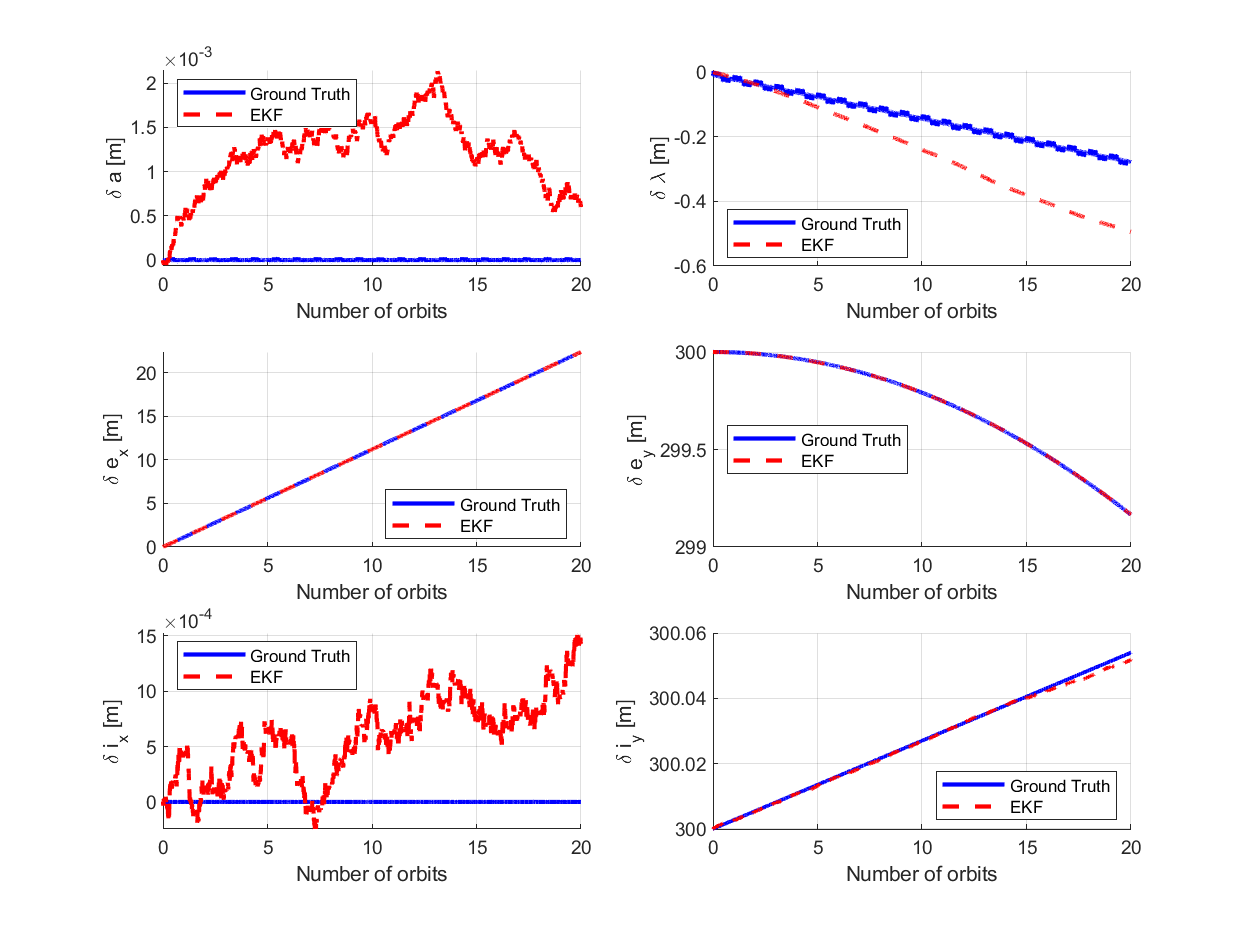
\includegraphics[width=0.8\linewidth]{sim/figures/PS8/ROE_over_time_SV2_comparison.png}
    \caption{Ground truth and EKF estimates for SV2 over time.}
    \label{fig:sv2_ekf_estimates}
\end{figure}

Figures \ref{fig:sv2_ekf_estimates_zoom} and \ref{fig:sv3_ekf_estimates_zoom} provide a closer look at the convergence behavior early in the simulation. Most states converge to reasonable error within the first orbit. This may be too slow for accurate control to be implemented in the loop, and so future work will look into faster convergence in the error. It is also clear that convergence is still not great in $i_x$ and $i_y$, which we hope to fix with further tuning.

\begin{figure}[H]
    \centering
    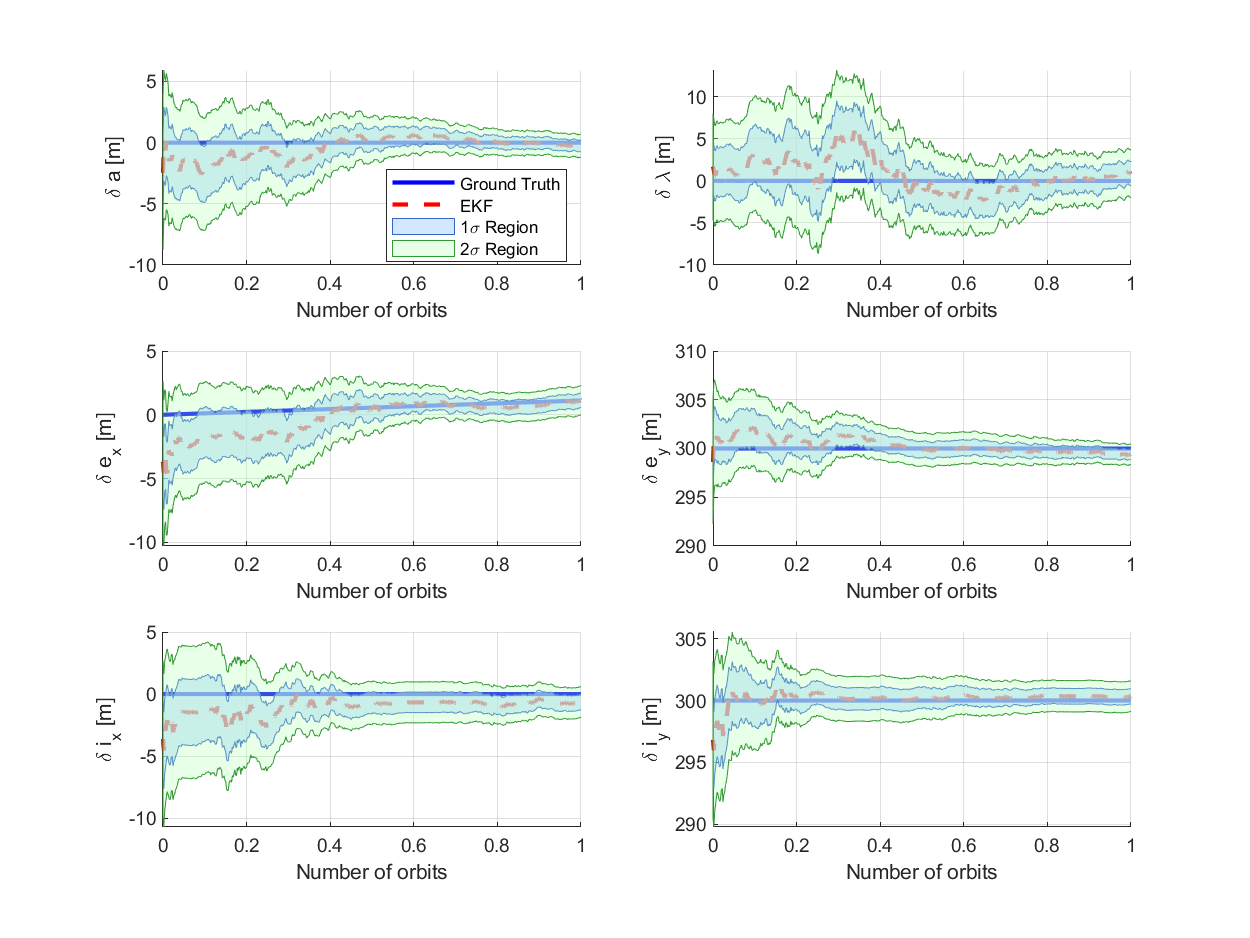
\includegraphics[width=0.8\linewidth]{sim/figures/PS8/ROE_over_time_SV2_comparison_zoomed.png}
    \caption{Ground truth and EKF estimates for SV2 over time, Zoomed-in view over the first orbit showing convergence for SV2.}
    \label{fig:sv2_ekf_estimates_zoom}
\end{figure}

\begin{figure}[H]
    \centering
    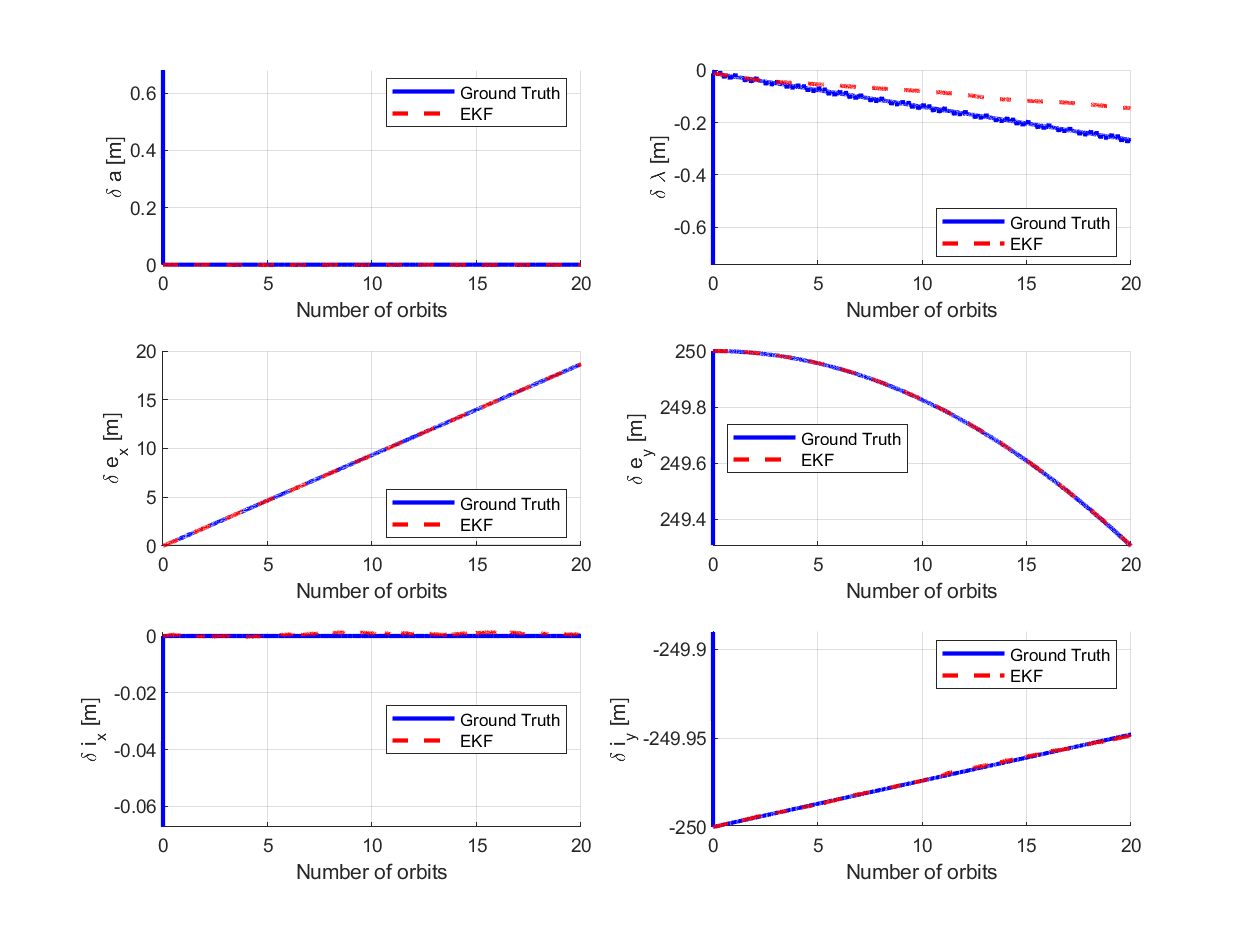
\includegraphics[width=0.7\linewidth]{sim/figures/PS8/ROE_over_time_SV3_comparison.png}
    \caption{Ground Truth and EKF estimates for SV3 over time}
    \label{fig:sv3_ekf_estimates}
\end{figure}

\begin{figure}[H]
    \centering
    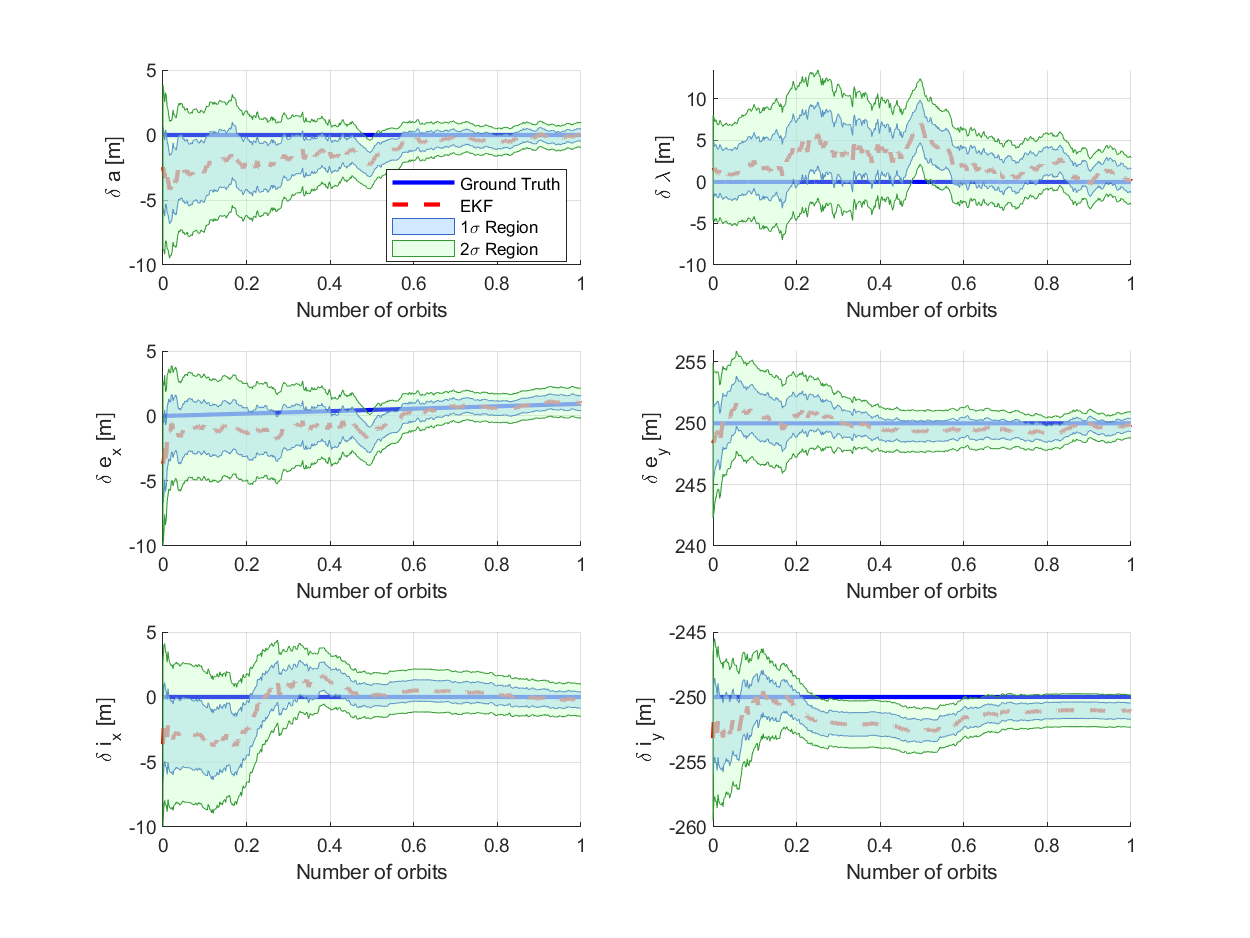
\includegraphics[width=0.7\linewidth]{sim/figures/PS8/ROE_over_time_SV3_comparison_zoomed.png}
    \caption{Ground Truth and EKF estimates for SV3, Zoomed version to first orbit, showing convergence.}
    \label{fig:sv3_ekf_estimates_zoom}
\end{figure}

Figures \ref{fig:sv2_ekf_error}, \ref{fig:sv2_ekf_error_zoomed}, \ref{fig:sv3_ekf_error}, and \ref{fig:sv3_ekf_error_zoomed} show the error in the EKF estimate with confidence bounds for SV2 and SV3. As expected, the errors and the confidence bounds decrease as more measurements are taken and the filter gets closer to the ground truth. The errors are all contained within the 2-sigma confidence bounds, which validates our posterior estimate distribution. Once again, the error convergence in $i_x$ and $i_y$ is poor, and is scope for future work.

Interestingly, the confidence bounds in $\delta \lambda$ increase before they decrease, which is unlike all the other ROEs. This is likely due to the dependence of $\delta \lambda$ and its drift on $\delta a$, $\delta i_x$, which have errors themselves. As such, it takes longer for the uncertainty in $\delta \lambda$ to decrease. 

\begin{figure}[H]
    \centering
    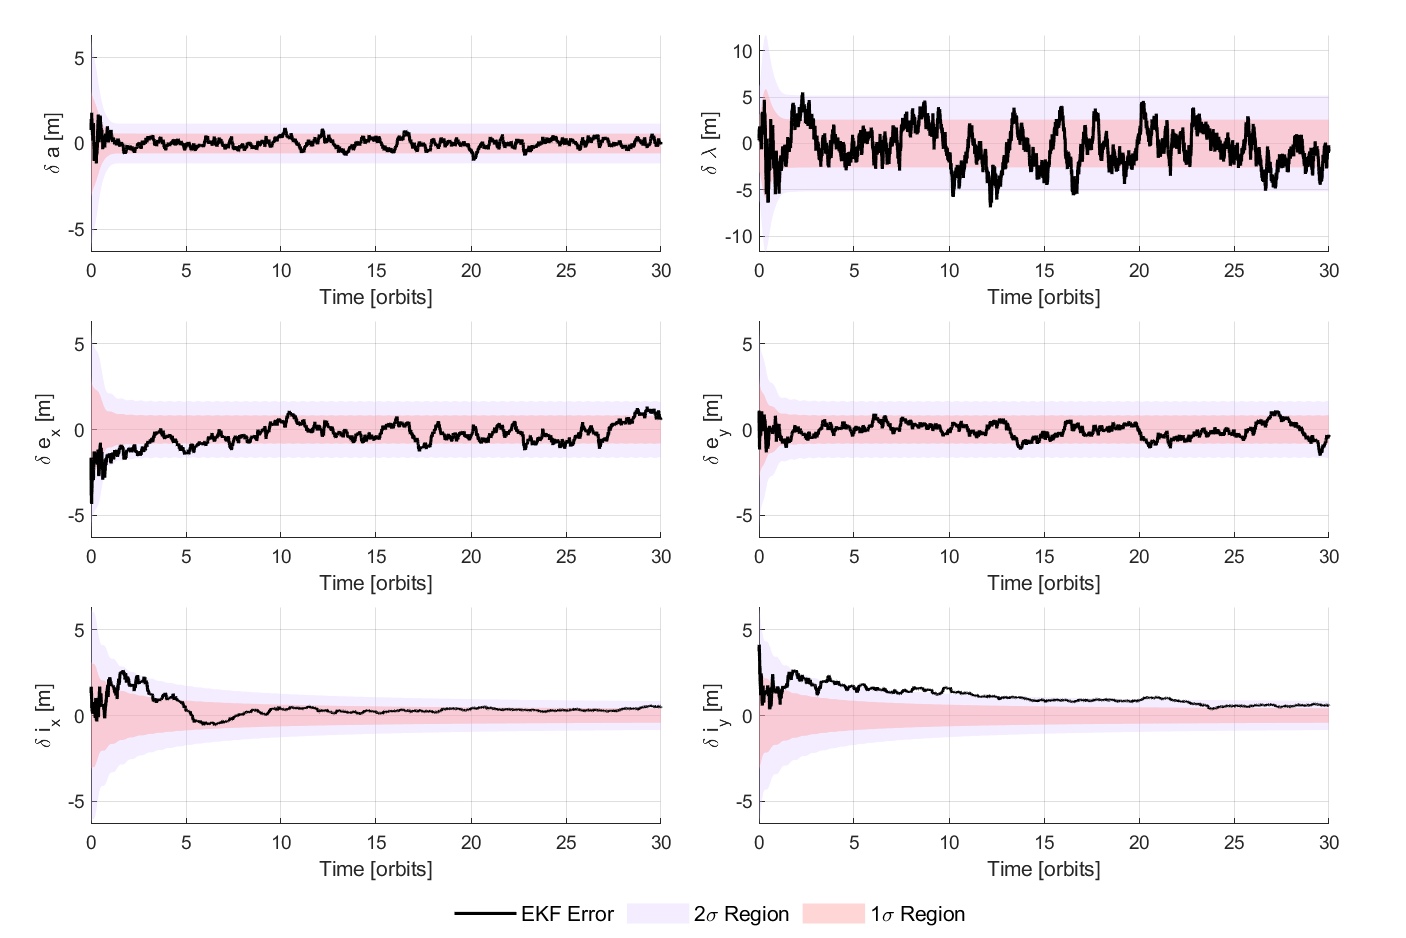
\includegraphics[width=0.7\linewidth]{sim/figures/PS8/EKF_error_SV2.png}
    \caption{Error in EKF estimates for SV2 over time}
    \label{fig:sv2_ekf_error}
\end{figure}

\begin{figure}[H]
    \centering
    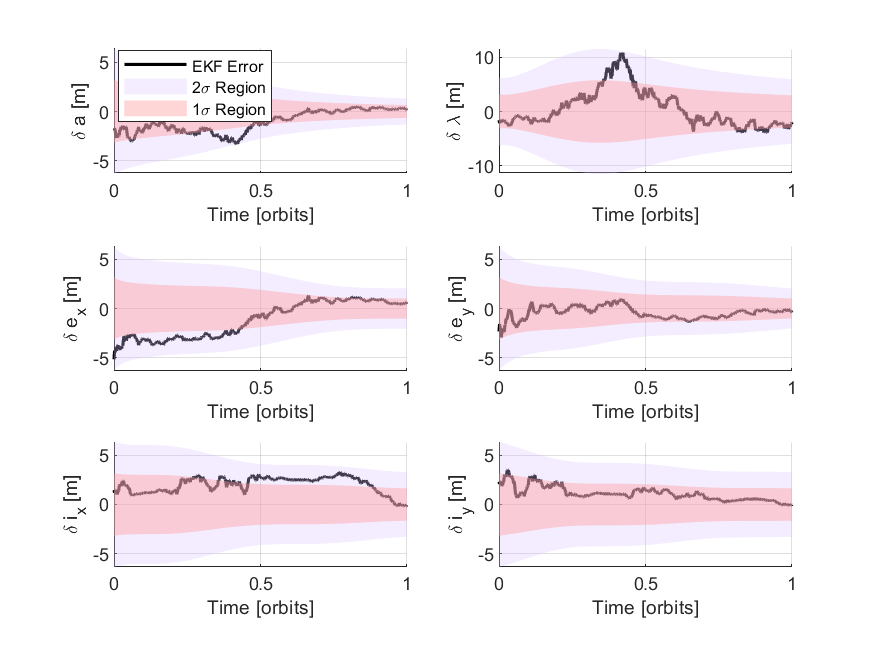
\includegraphics[width=0.7\linewidth]{sim/figures/PS8/EKF_error_SV2_zoomed.png}
    \caption{Error in EKF estimates for SV2 over time, zoomed to the first orbit to show convergence}
    \label{fig:sv2_ekf_error_zoomed}
\end{figure}

\begin{figure}[H]
    \centering
    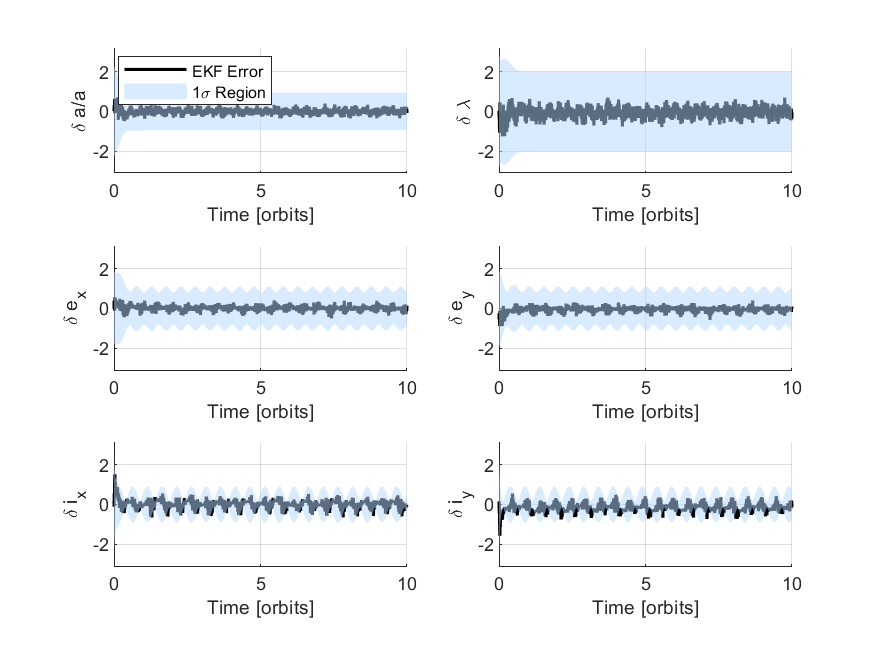
\includegraphics[width=0.7\linewidth]{sim/figures/PS8/EKF_error_SV3.png}
    \caption{Error in EKF estimates for SV3 over time}
    \label{fig:sv3_ekf_error}
\end{figure}

\begin{figure}[H]
    \centering
    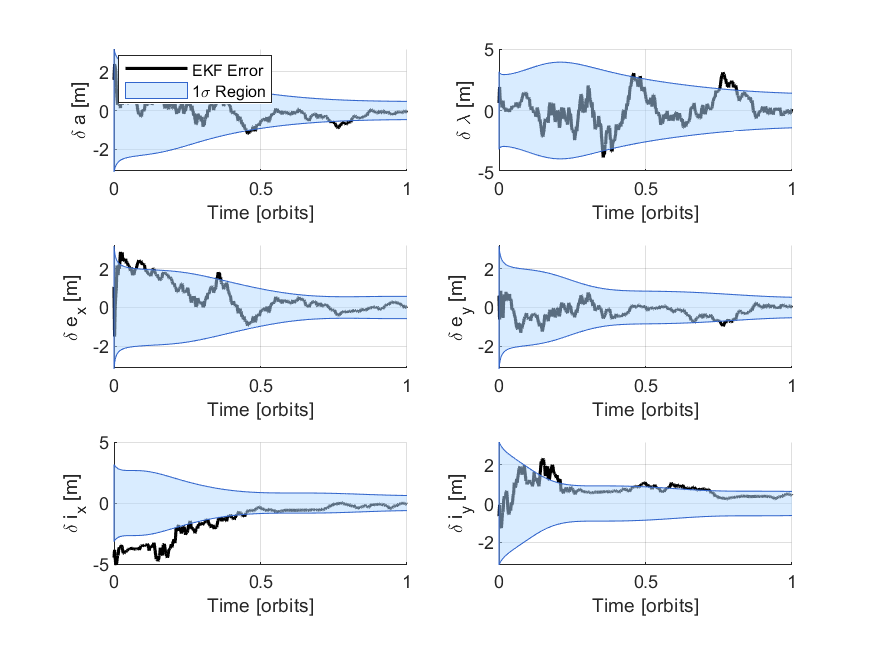
\includegraphics[width=0.7\linewidth]{sim/figures/PS8/EKF_error_SV3_zoomed.png}
    \caption{Error in EKF estimates for SV3 over time, zoomed to the first orbit to show convergence}
    \label{fig:sv3_ekf_error_zoomed}
\end{figure}

Figures \ref{fig:sv2_residuals} and \ref{fig:sv3_residuals} show the pre-fit and post-fit residuals for SV2 and SV3 by comparing the predicted and updated measurements with the true measurements. As expected, the post-fit residuals are smaller than the pre-fit residuals, which shows that the filter is updating the estimate to be closer to true state based on the difference in predicted and true measurements. The difference between the pre-fit and post-fit residuals being small is a consequence of a small $Q$ value and a relatively large $R$ value, which reduces the change in the residual during the measurement step. 

Additionally, the residuals are on the same scale as the injected measurement noise, which is also expected. In a well-tuned EKF, the post-fit residuals reflect the injected noise once the state estimate has accounted for dynamic and measurement uncertainties. 

\begin{figure}[H]
    \centering
    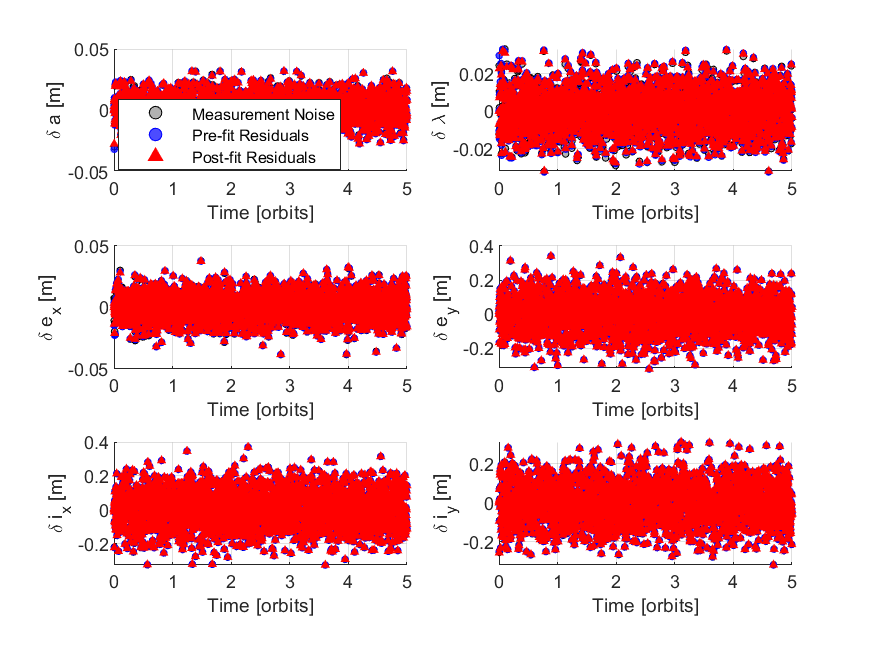
\includegraphics[width=0.7\linewidth]{sim/figures/PS8/residuals_SV2.png}
    \caption{Pre-fit and post-fit residuals in SV2}
    \label{fig:sv2_residuals}
\end{figure}

\begin{figure}[H]
    \centering
    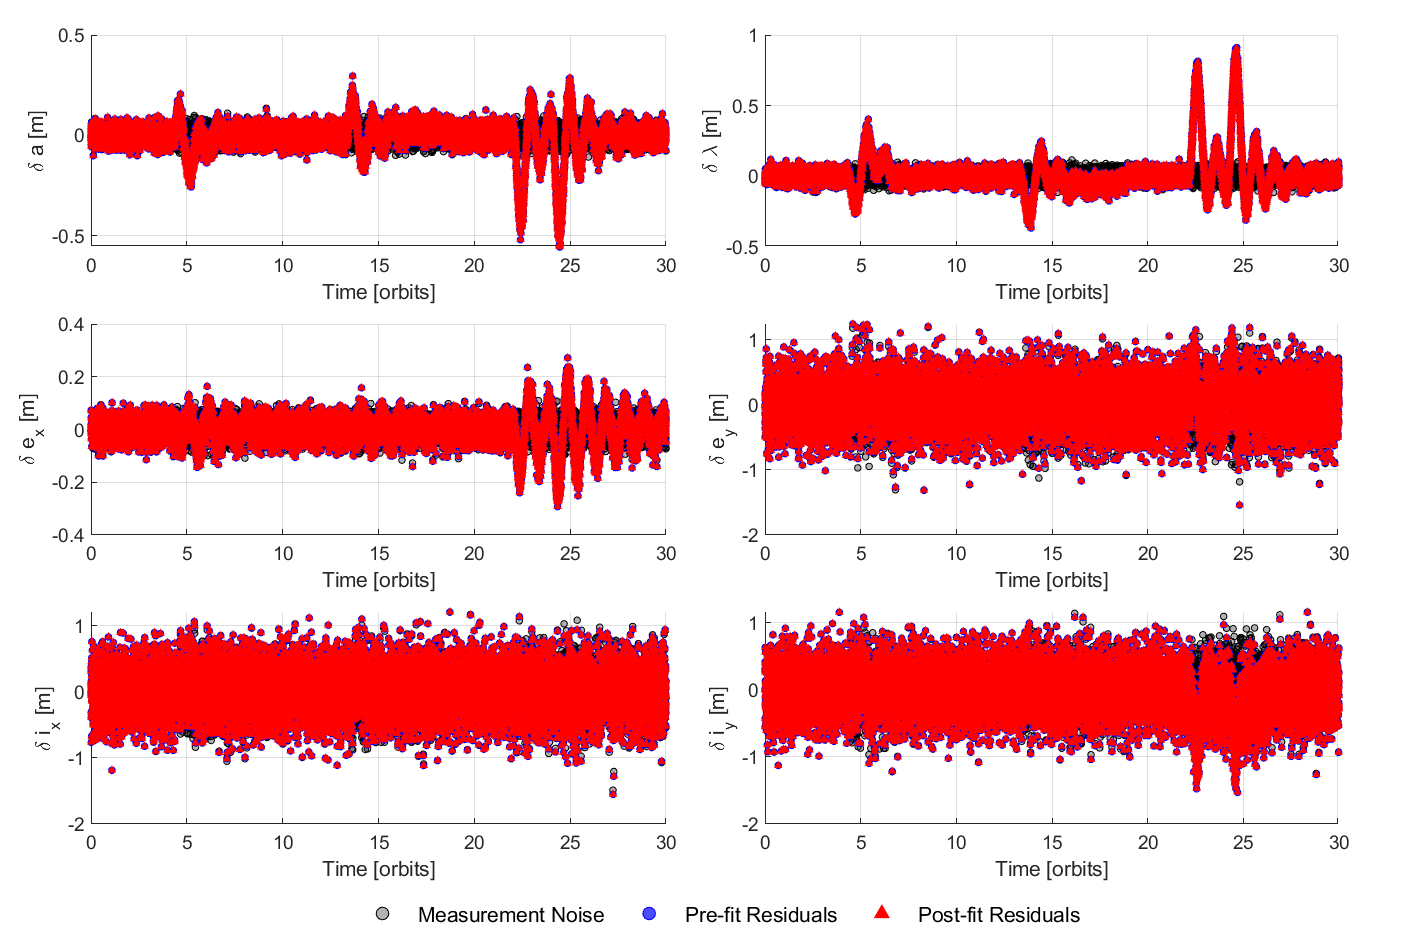
\includegraphics[width=0.7\linewidth]{sim/figures/PS8/residuals_SV3.png}
    \caption{Pre-fit and post-fit residuals in SV3}
    \label{fig:sv3_residuals}
\end{figure}

Finally, as a metric of performance we can also look at the mean and standard deviation of the state error at the end of the simulation. For the standard deviation in the state, we utilize the diagonal elements of our final covariance matrices and take the square root of those quantiies. These metrics for SV2 and SV3 are reported in $m$ below.


\begin{align}
    \mu_{err, SV2} &= \begin{bmatrix} 0.183 \\ -3.418 \\ 1.015 \\ 0.315 \\ 0.177 \\ -0.091 \end{bmatrix} m\\
    \sigma_{err, SV2} &= \begin{bmatrix} 0.578 \\ 2.579 \\ 0.816 \\ 0.824 \\ 0.631 \\ 0.632 \end{bmatrix} m\\
    \mu_{err, SV3} &= \begin{bmatrix} 0.043 \\ 0.953 \\ -0.202 \\ -0.857 \\ -0.275 \\ -0.405 \end{bmatrix} m\\
    \sigma_{err, SV3} &= \begin{bmatrix} 0.578 \\ 2.579 \\ 0.816 \\ 0.824 \\ 0.631 \\ 0.632 \end{bmatrix} m
\end{align}

These values, which are all in meters, are orders of magnitude smaller than our state (scaled relative orbital elements for our systems are in $100$s of meters). Notably, due to the dependence of $\delta \lambda$ on the estimates of other states, its uncertainty is generally higher than that of the other states.